% -*- root: ../../main.tex -*-
\section{Mediator}
\label{sec:mediator_design}

Dopo un attento studio delle \textbf{specifiche} sviluppate nella fase di analisi è emerso un importante \textbf{problema di interazione} fra alcuni \textbf{componenti cardine}. Come è stato ribadito in \ref{subsec:client_server} il design è stato sviluppato cercando di tenere conto dei principali \textbf{requisiti di qualità} e \textbf{buona progettazione}. Questo grado di \textbf{estendibilità} e \textbf{modularizzazione} si è esplicitato nella defini-zione di una architettura (\texttt{Core}) \textbf{espandibile a richiesta} verso un modello \textbf{client-server} ad \textbf{attori} (\texttt{Core + Actor}).

Mantenere un \textbf{core unico} e \textbf{polifunzionale} non è semplice ed è necessario ridefinire gli elementi mobili utilizzando il cosidetto \texttt{loose coupling}. 

\subsection{Il problema}
Nell'architettura core definita in fase di progettazione il problema risiede essenzialmente nella gestione del passaggio da \textbf{single-player} game a \textbf{multiplayer}. 

\paragraph{Single-player:}
Nella versione single-player il sistema di gioco si appoggia sul cosiddetto \texttt{GameEngine} il quale è in grado di \textbf{calcolare autonomamente gli aggiornamenti} da inviare alla/e schermata/e di gioco.

\paragraph{Multiplayer:}
Nel caso multiplayer esiste un \textbf{server unico} a cui sono collegati una serie di \textbf{client}. Il server agisce da \textbf{leader} poiché, possedendo un \texttt{GameEngine} proprio, è in grado di calcolare gli \textbf{aggiornamenti di gioco} a fronte di \textbf{input propri} e \textbf{dei client}. I client, al fine di promuovere \textbf{semplicità}, sono stati concepiti come \textbf{architetture core} private del motore di calcolo \texttt{GameEngine}. Essi in poche parole si presentano come \textbf{attori passivi} che \textbf{acquisiscono aggiornamenti} dal server e li mostrano all'utente attraverso una \textbf{interfaccia grafica}.

Un approccio di questo tipo è molto utile poiché permette di poter utilizzare il server per giocare \textbf{ospitando contemporaneamente la partita in corso}. Inoltre promuove \textbf{leggerezza} e \textbf{riusabilità} dato che i client devono mostrare le \textbf{stesse informazioni} che il server produrrebbe per sé stesso in modalità single-player.

\paragraph{Da Single-player a Multiplayer:}
Il problema, come abbiamo detto, si presenta nel passaggio dalla modalità \textbf{single-player} a quella \textbf{multiplayer}. Nel caso di un passaggio a \textbf{server-mode} il sistema dovrà mantenere il core intatto ma dovrà aver cura di \textbf{inviare gli aggiornamenti} non solo all'\textbf{interfaccia locale} ma anche all'\textbf{attore server} (il quale effettuerà un broadcast ai client). Il passaggio a \textbf{client-mode} è ancora più delicato; in questo caso, infatti, sarà necessario spegnere il modulo \texttt{GameEngine} \textbf{dirottando i flussi di informazione} verso il \textbf{client-actor}.

\subsection{La soluzione}
\label{subsec:mediator_solution}
Al fine di definire una soluzione valida ci si è appoggiati su un pattern di design di tipo comportamentale, il \textbf{pattern Mediator}. Il pattern consiste nella definizione di un \textbf{modulo} esterno a tutti gli altri il cui scopo consiste essenzialmente nella \textbf{mediazione e ridirezionamento dei flussi} di dati.

Nel nostro caso il Mediator ha lo scopo principe di \textbf{mediare le interazioni} fra quattro componenti fondamentali:
\begin{itemize}
	\item{\textbf{Schermata di gioco:}}
	Deve essere in grado di inviare comandi al \textbf{proprio}  \texttt{GameEngine} (single-player) oppure al \texttt{GameEngine} \textbf{del server} (multiplayer). 
	\item{\textbf{Engine:}}
	Riceve i comandi dal proprio \texttt{GameScreen} (single-player) o dai \texttt{GameScreen} dei client e li elabora producendo un \textbf{nuovo aggiornamento}. 
	\item{\textbf{Attore Client:}}
	Può essere concepito come un \texttt{Core} munito solo di un unico \texttt{GameScreen}.
	\item{\textbf{Attore Server:}}
	Può essere concepito come un \texttt{Core} agganciato a un numero di \texttt{GameScreen} variabile.
\end{itemize}
Al fine di gestire al meglio le interazioni è stato scelto di implementare un \textbf{approccio basato su eventi} che è stato poi pensato in \textbf{due versioni molto simili}:
\begin{itemize}
	\item{\textbf{Mediator Handler:}}
	Il \textbf{Mediator} è stato progettato sfruttando il \textbf{pattern ad handler} basato su \textbf{eventi}.
	\item{\textbf{Mediator Observer:}}
	Il \textbf{Mediator} è stato progettato sfruttando il \textbf{pattern observer ad eventi}.
\end{itemize}

Come vediamo in figura \ref{fig:mediatorHandler} la prima scelta porta come principale vantaggio l'ottenimento di \textbf{performance migliori} poiché ogni handler rappresenta del \textbf{codice associato ad un evento immediatamente eseguibile}. A questo però si aggiungono una \textbf{serie di problematiche} (vedi \ref{subsubsec:mediator_handler_problem}) che hanno portato a rivedere la soluzione proposta dirigendosi verso un'altra soluzione.
\begin{figure}[H]
	\centering
	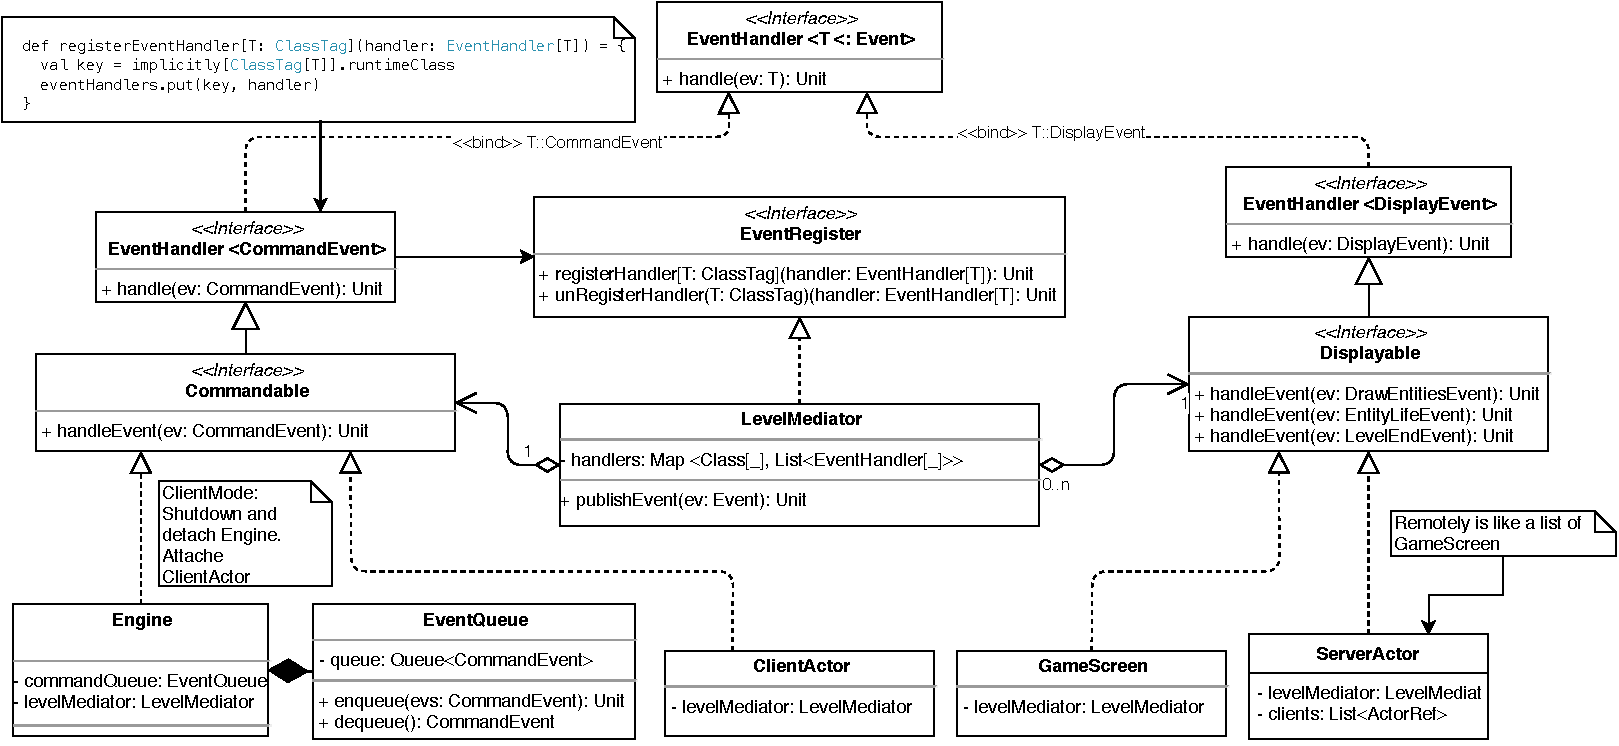
\includegraphics[width=0.99\columnwidth]{drawio/mediator/mediatorHandler.pdf}
	\caption{Design del Mediator basato su handlers.}
	\label{fig:mediatorHandler}
\end{figure}

La versione basata su handler è stata quindi rivista in un \textbf{approccio} maggiormente \textbf{strutturato} incentrato principalmente sul \textbf{Pattern Observer ad eventi}. (fig: \ref{fig:mediatorObserver}).
\begin{figure}[H]
	\centering
	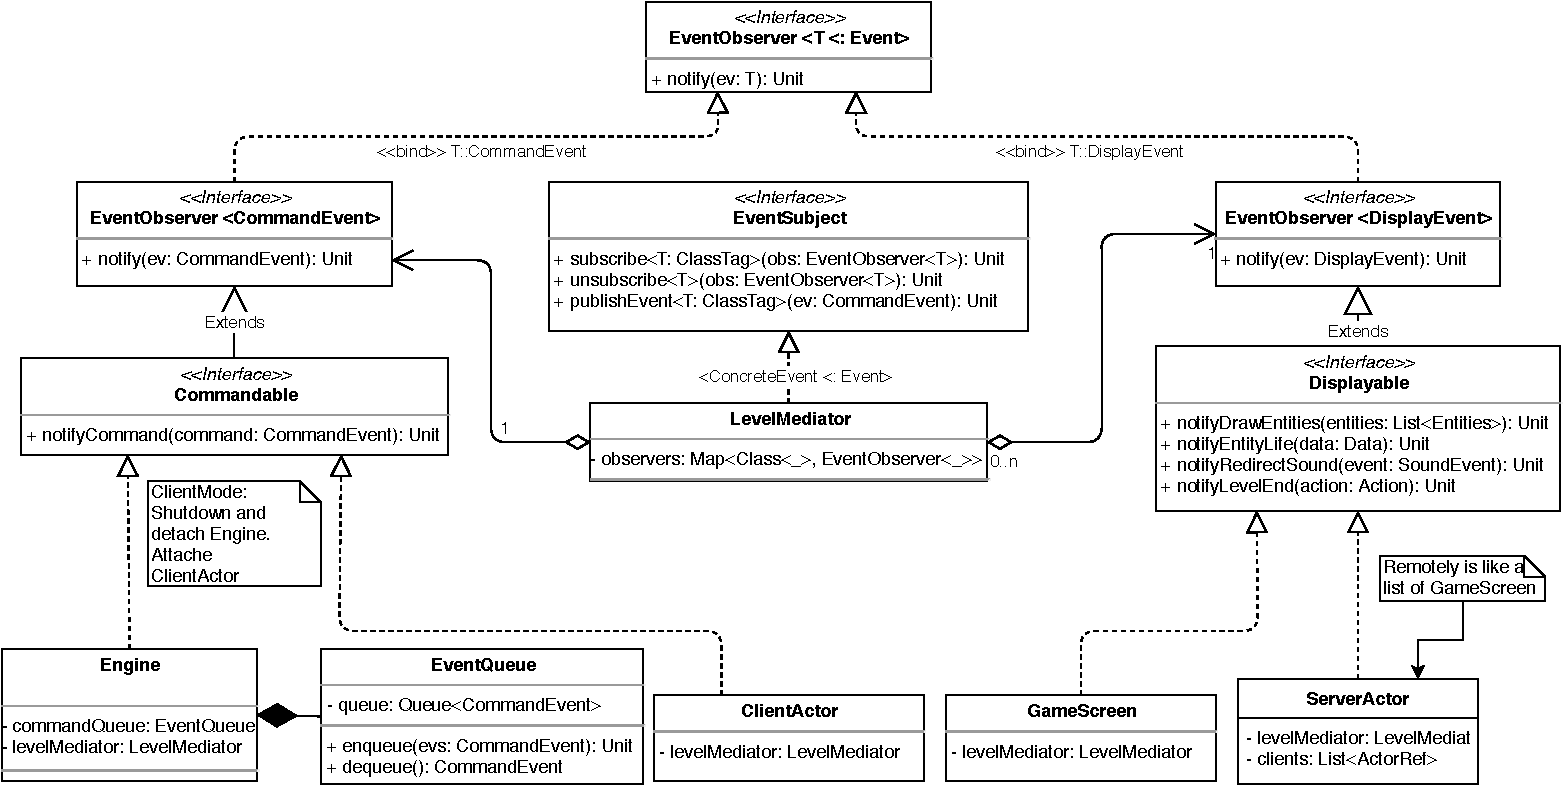
\includegraphics[width=0.99\columnwidth]{drawio/mediator/mediatorObserver.pdf}
	\caption{Design del Mediator basato su observer.}
	\label{fig:mediatorObserver}
\end{figure}

\subsection{Funzionamento}

La presenza del \textbf{\texttt{Mediator}} gioca un ruolo fondamentale nel \textbf{riuso} del codice perché, come approfondito in \ref{subsec:mediator_solution} permette di \textbf{passare in maniera semplice} dalla modalità single-player a quella multi-player e viceversa.

Il diagramma di \textbf{sequenza}, raffigurato in \ref{fig:sequenceMediator} mostra le dinamiche delle \textbf{interazioni} che coinvolgono il \texttt{Mediator} nel caso in cui ci si trovi nella modalità di gioco \textbf{multiplayer} e che, di conseguenza, siano coinvolti \textbf{Client} e \textbf{Server}.

\begin{figure}[H]
	\centering
	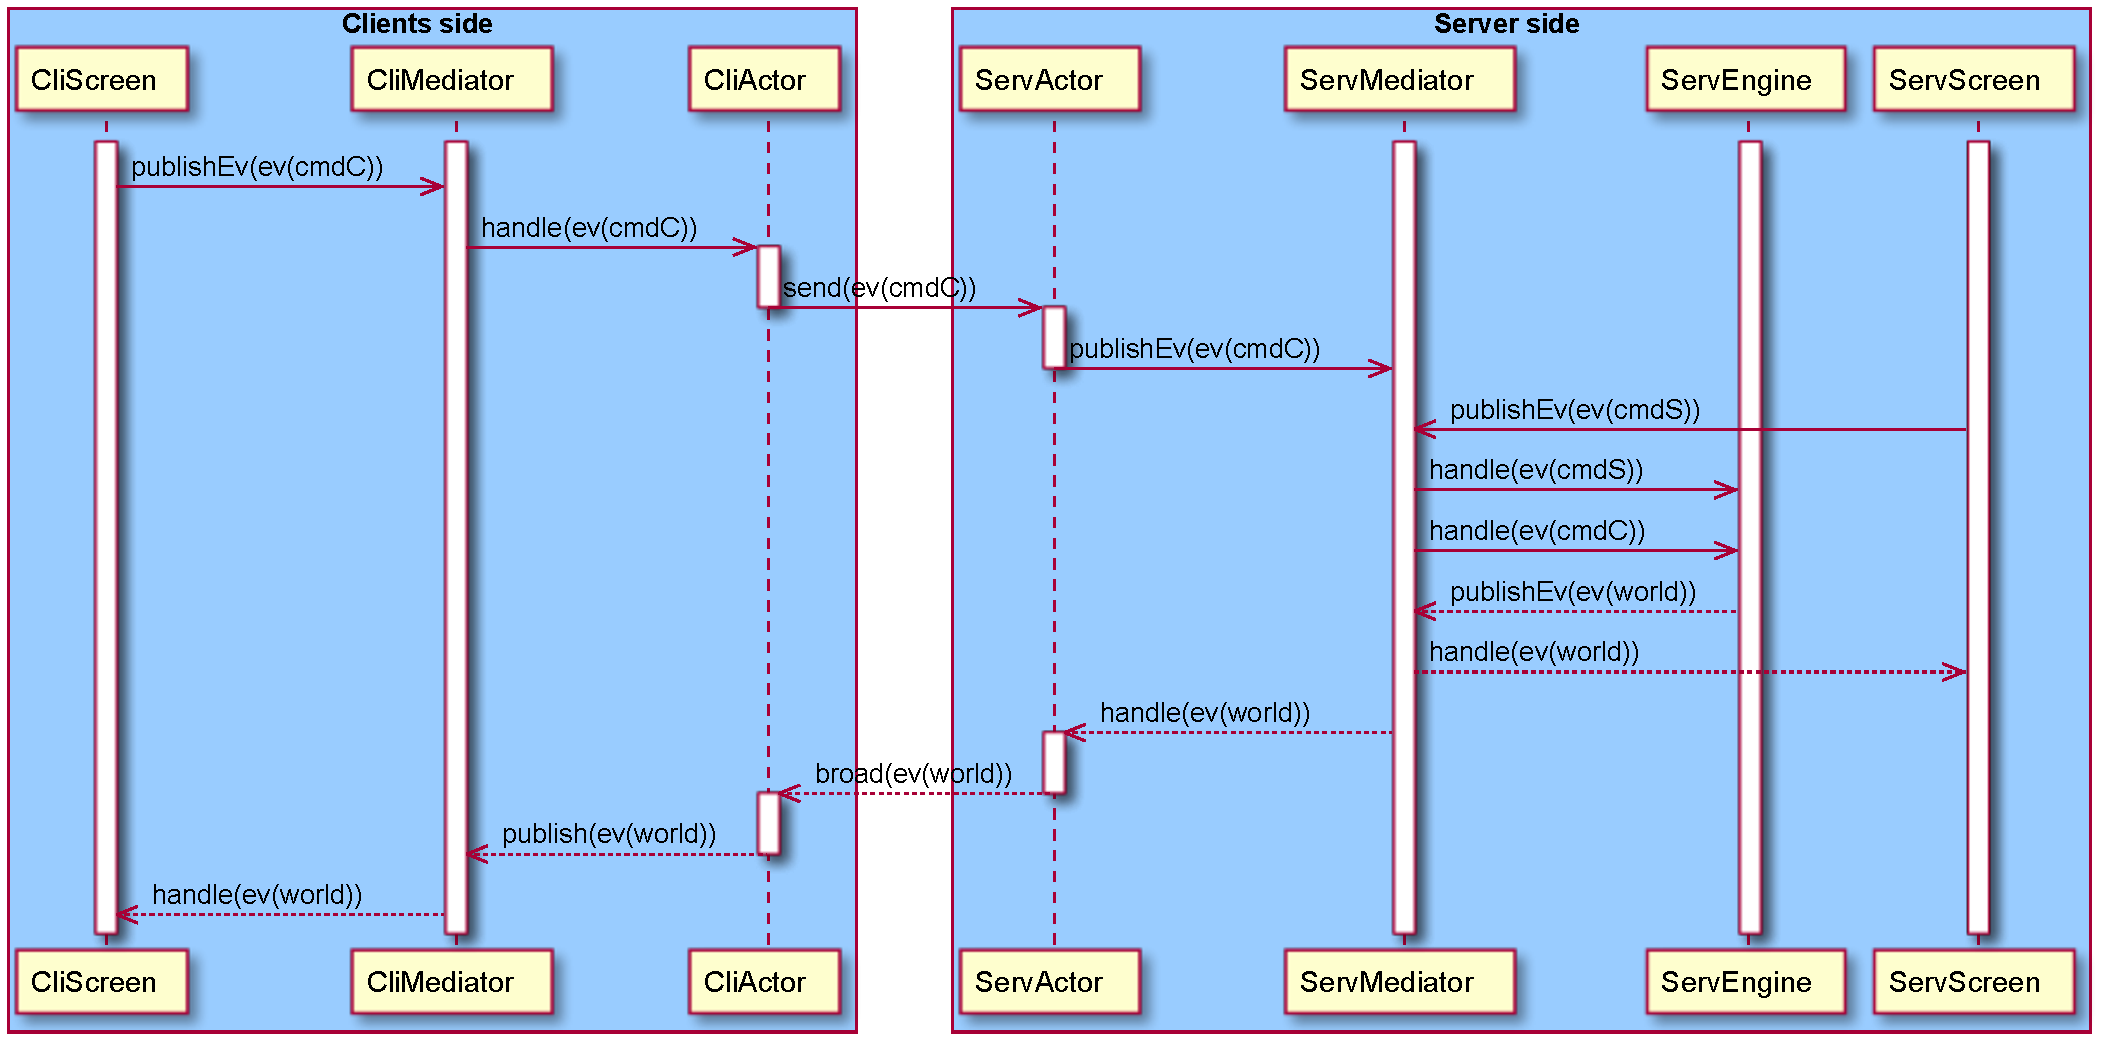
\includegraphics[width=0.99\columnwidth]{plantuml/rendered/sequenceDiagrams/sequenceMediator.pdf}
	\caption{Diagramma di sequenza di un ciclo di comunicazione Client-Server.}
	\label{fig:sequenceMediator}
\end{figure}

Partendo dal messaggio immediatamente successivo allo start della partita si avranno, in maniera \textbf{iterativa}, le seguenti interazioni:
    \begin{enumerate}
        \item Il \textbf{Client} avrà appena ricevuto il \textbf{mondo di gioco} e sarà in \textbf{attesa dell'input} generato dalla reazione del giocatore. 
        Il \texttt{GameScreen} rileva il comando e \textbf{pubblica} il relativo evento verso il proprio \textbf{Mediator}
        \item Il \texttt{Mediator} del \textbf{Client} procede a \textbf{propagare} l'evento a tutti coloro che sono ad esso \textbf{sottoscritti}. Nel caso del Client, solo il \textbf{\texttt{ClientActor}}.
        \item Il \texttt{ClientActor}, ricevuto l'evento, lo comunicherà al \texttt{ServerActor} che procederà con la \textbf{pubblicazione} sul proprio \texttt{\textbf{Mediator}}
        \item Il \texttt{Mediator} del \textbf{Server} propaga l'evento ricevuto a tutti gli interessati. L'unico ad essere sottoscritto, nel caso del Server è l'\texttt{Engine}.
        \item Il \texttt{GameScreen} del \textbf{Server} cattura il \textbf{comando} del giocatore che ospita alla partita. Questo comando, come accadeva per il Client, viene inoltrato al \texttt{\textbf{Mediator}} di riferimento.
        \item Il \texttt{Mediator} invia a questo punto il comando all'\texttt{Engine} 
        \item L'\texttt{Engine}, a questo punto, potrà calcolare il \textbf{nuovo mondo di gioco}, basandosi sulle azioni dell'\textbf{Intelligenza Artificiale} e dei \textbf{giocatori}, e inviarlo al proprio \texttt{Mediator} di riferimento.
        \item In conclusione il \texttt{Mediator} invia il messaggio al \texttt{GameScreen} di tutti i giocatori: al Server in maniera diretta e ai Client tramite il layer di comunicazione.
    \end{enumerate}
\paragraph{Single-player} Nella modalità single-player si mantengono le dinamiche principali, ma senza tenere conto del layer di comunicazione dato da \texttt{ClientActor} e \texttt{ServerActor} poiché in tale modalità non sono presenti. Le interazioni principali avverranno quindi tra \texttt{GameScreen}, \texttt{Mediator} e \texttt{Engine}, nelle stesse modalità riportate precedentemente.

